\documentclass[tikz,border=5pt]{standalone}
\usepackage{amsmath}
\begin{document}
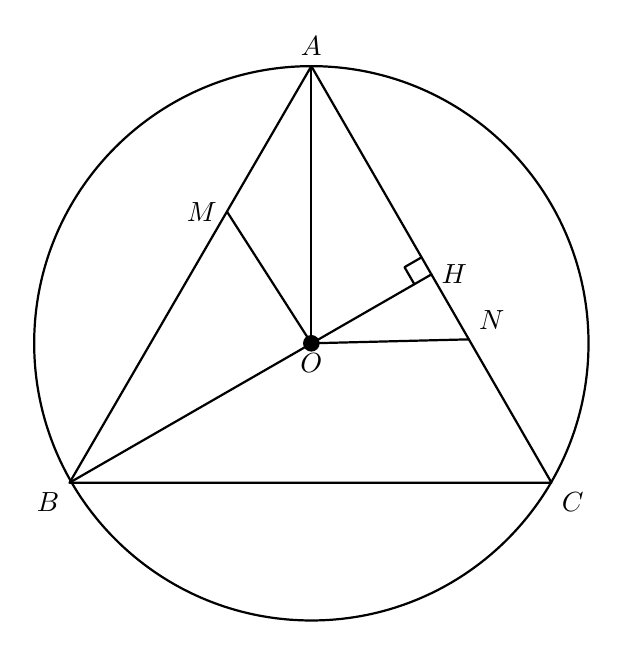
\begin{tikzpicture}[scale=1, line cap=round, line join=round, thick]
  % 坐标定义
  \coordinate (O) at (3.69,0);
  \coordinate (A) at (3.69,3.52);
  \coordinate (B) at (0.62,-1.77);
  \coordinate (C) at (6.74,-1.77);
  \coordinate (M) at (2.62,1.67);
  \coordinate (N) at (5.69,0.05);
  \coordinate (H) at (5.215,0.875);

  % 外接圆
  \draw (O) circle (3.52);

  % 三角形
  \draw (A) -- (B) -- (C) -- cycle;

  % 半径 AO，OM，ON
  \draw (A) -- (O);
  \draw (O) -- (M);
  \draw (O) -- (N);

  % 新增：从 B 向 AC 作垂线 BH
  \draw (B) -- (H);

  % 直角标记
  \draw (5.09,1.092) -- (4.8735,0.967) -- (4.9985,0.75);

  % 点与标签
  \fill (O) circle (3pt);
  \node[above] at (A) {$A$};
  \node[below left] at (B) {$B$};
  \node[below right] at (C) {$C$};
  \node[left] at (M) {$M$};
  \node[above right] at (N) {$N$};
  \node[below] at (O) {$O$};
  \node[right] at (H) {$H$};
\end{tikzpicture}
\end{document}
